\documentclass{standalone}
\usepackage{tikz}
\usetikzlibrary{shapes,arrows,positioning,fit,calc}
% First declare a background layer if not already done
\pgfdeclarelayer{background}
\pgfsetlayers{background,main}


\begin{document}
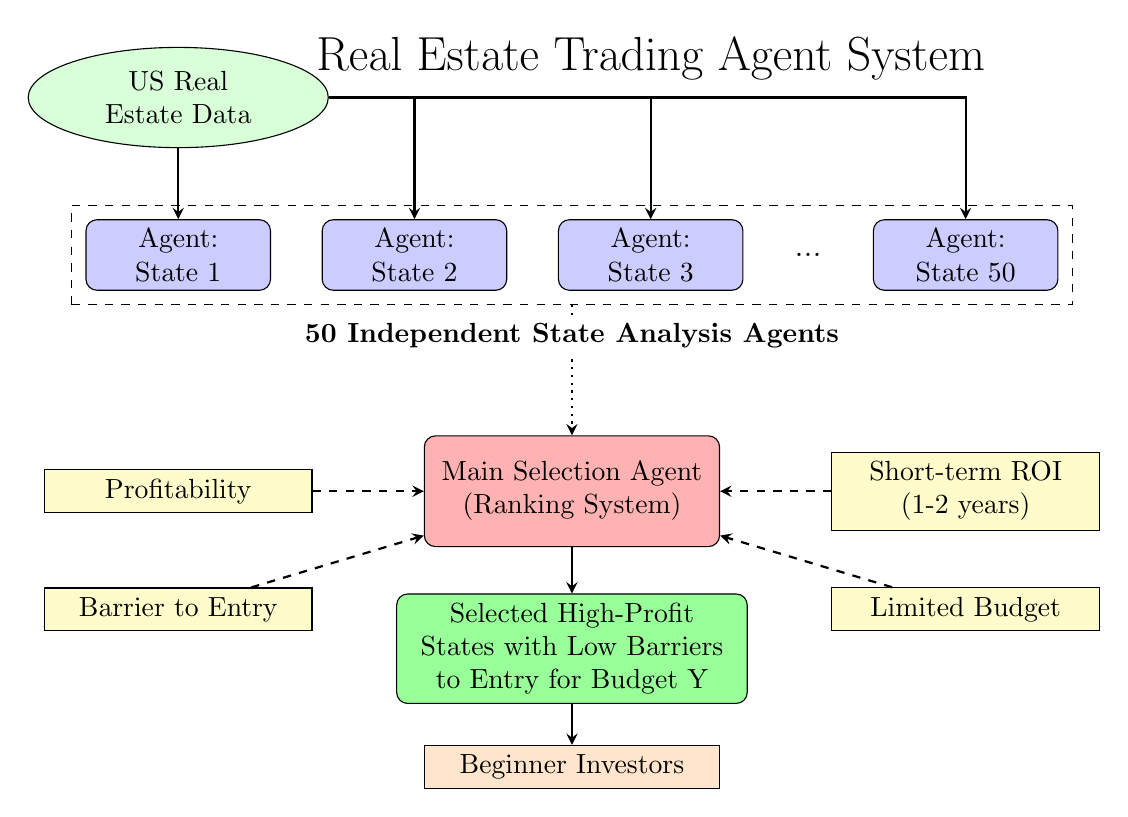
\begin{tikzpicture}[
    node distance=1.5cm,
    stateagent/.style={rectangle, draw, fill=blue!20, text width=6em, text centered, rounded corners, minimum height=2.5em},
    mainagent/.style={rectangle, draw, fill=red!30, text width=10em, text centered, rounded corners, minimum height=4em},
    datanode/.style={ellipse, draw, fill=green!15, text width=7em, text centered},
    arrow/.style={thick,->,>=stealth},
    box/.style={rectangle, draw, dashed, inner sep=0.5em},
    criteria/.style={rectangle, draw, fill=yellow!20, text width=9em, text centered}
]

% Title

\node[text centered] at (0,3.5) {\LARGE Real Estate Trading Agent System};


% Data sources
\node[datanode] (data) at (-6,3) {US Real Estate Data};

% State agents (showing a representative sample)
\node[stateagent] (s1) at (-6,1) {Agent: State 1};
\node[stateagent] (s2) at (-3,1) {Agent: State 2};
\node[stateagent] (s3) at (0,1) {Agent: State 3};
\node at (2,1) {\large ...};
\node[stateagent] (s50) at (4,1) {Agent: State 50};

% Data flowing to agents
\draw[arrow] (data) -- (s1);
\draw[arrow] (data) -| (s2);
\draw[arrow] (data) -| (s3);
\draw[arrow] (data) -| (s50);

% Group the state agents
\node[box, fit=(s1) (s2) (s3) (s50), label={below:{\colorbox{white}{\textbf{50 Independent State Analysis Agents}}}}] (agentbox) {};

% Main selection agent
\node[mainagent] (main) at (-1,-2) {Main Selection Agent\\(Ranking System)};


% Connect state agents box to main agent

% Then in your tikzpicture code:
\begin{pgfonlayer}{background}
    \draw[arrow, dotted] (agentbox.south) -- (main.north);
\end{pgfonlayer}


% Connect state agents to main agent
%\foreach \i in {s1,s2,s3,s50}
%    \draw[arrow] (\i) -- (\i |- main.north);

% Selection criteria
\node[criteria] (c1) at (-6,-2) {Profitability};
\node[criteria] (c2) at (-6,-3.5) {Barrier to Entry};
\node[criteria] (c3) at (4,-2) {Short-term ROI\\(1-2 years)};
\node[criteria] (c4) at (4,-3.5) {Limited Budget};

\draw[arrow, dashed] (c1) -- (main);
\draw[arrow, dashed] (c2) -- (main);
\draw[arrow, dashed] (c3) -- (main);
\draw[arrow, dashed] (c4) -- (main);

% Output: Selected states
\node[rectangle, draw, fill=green!40, text width=12em, text centered, rounded corners] (output) at (-1,-4) {Selected High-Profit States with Low Barriers to Entry for Budget Y};
\draw[arrow] (main) -- (output);

% Target audience
\node[rectangle, draw, fill=orange!20, text width=10em, text centered] (audience) at (-1,-5.5) {Beginner Investors};
\draw[arrow] (output) -- (audience);

% Adaptability option
%\node[rectangle, draw, dashed, fill=purple!10, text width=10em, text centered] (adapt) at (7,3) {Adaptability Option:\\Different Countries};
%\draw[arrow, dashed] (adapt) |- (main);

\end{tikzpicture}
\end{document}
